\section{The EnD regularization}
\label{sec:supervised-end}



\begin{table}
   \center
    \caption{Overview on the notation used in this work.}
    \begin{tabular}{c l}%
        \toprule
        \textbf{Symbol} & \textbf{Meaning}\\
        \midrule
        $x_i$      & input ($i$-th sample in the dataset)\\
        $y_i$      & predicted class for the $i$-th sample \\
        $t_i$      & target class for the $i$-th sample \\
        $b_i$      & bias class for the $i$-th sample \\
        
        $Y$        & random variable associated to the predicted labels\\
        $T$        & random variable associated to the target labels\\
        $B$        & random variable associated to the bias labels\\
        $N_T$                     & cardinality of targets\\
        
        
        
        
        
        
      
        
        \bottomrule
    \end{tabular}
    \label{tab:notationover}
\end{table}

In this section we introduce the notation we adopt in this work, and provide a detailed explanation on how the EnD~\cite{tartaglione2021end} debiasing technique works in a supervised setting. Then, in Sec.~\ref{sec:unsupervised-end} we will move on to the unsupervised extension. 
The notation introduced in this work is summarized in Table~\ref{tab:notationover}\footnote{for the rest of this work, we conform to the standard notation proposed by Goodfellow~\emph{et~al.}~\cite{GoodBengCour16}, available at \url{https://github.com/goodfeli/dlbook\_notation}}.
Given a neural network \emph{encoder} $f(\cdot) \in R^N$ %
which extracts feature vectors of size $N$ and a \emph{classifier} $g(\cdot) \in R^{N_T}$ which provides the final prediction, we consider the neural network $(g~\circ~\gamma~\circ~f)(\cdot)$
where $\gamma : \mathbb{R}^N \rightarrow \mathbb{R}^N$ is a normalization function to obtain $z = \gamma(x) = x/\|x\|_2$.
The EnD regularization term $\mathcal{R}$ is applied jointly with the loss function $\mathcal{L}$ (e.g. cross-entropy), forcing $(\gamma \circ f)(\cdot)$ to filter out biased features from the extracted representation $z$. 
Hence, the overall objective function we aim to minimize is
\begin{equation}
    \label{eq:uprule}
    \mathcal{J} = \mathcal{L} + \mathcal{R},
\end{equation}
where $\mathcal{R}$ is the sum of the disentangling and entangling terms, weighted by two hyper-parameters $\alpha$ and $\beta$:
\begin{equation}
\label{eq:objective-func}
    \mathcal{R} = \alpha\mathcal{R}^{\perp} + \beta\mathcal{R}^{\parallel}
\end{equation}
Within a minibatch, let $i \in I \equiv \{1\dots M\}$ be the index of an arbitrary sample. We define $y_i$, $t_i$ and $b_i$ as the predicted, ground truth target and bias classes, respectively. 
The disentangling term $R^{\perp}$ is defined, for the $i$-th sample, as: 
\begin{equation}
	\mathcal{R}^{\perp}_{i} = \frac{1}{|B(i)|} \sum_{a \in B(i)} z_i \cdot z_a
\end{equation}
where $B(i) := \{j \in I \mid b_j = b_i  \} \setminus \{i\}$ is the set of all samples sharing the same bias class of $x_i$. 
The goal of this term is to suppress the common features among samples which have the same bias. %
The entangling term $R^{\parallel}$ is defined, for the $i$-th sample, as:
\begin{equation}
	\mathcal{R}^{\parallel}_{i} = - \frac{1}{|J(i)|}\sum_{j \in J(i)} z_i \cdot z_j
\end{equation}
where $J(i) := \{ j \in I \mid t_j = t_i \} \setminus B(i)$ is the set of all samples sharing the same target class of $x_i$ but with different biases. %
Complementarily to the disentangling term, the goal of this term is to encourage correlation among samples of the same class but with different bias, in order to introduce invariance with respect to the biased features.
So, for the $i$-th sample, the entire EnD regularization term $\mathcal{R}_i$ can be written as: 
\begin{equation}
\label{eq:end-full-new}
  \mathcal{R}_i =  \alpha\frac{1}{|B(i)|} \sum_{a \in B(i)} z_i \cdot z_a - \beta \frac{1}{|J(i)|}\sum_{j \in J(i)} z_i \cdot z_j \,. 
\end{equation}
The final $\mathcal{R}$ of Eq.~\ref{eq:objective-func}, is then just computed as the average over the minibatch: 

\begin{equation}
    \mathcal{R} = \frac{1}{M}\sum_i \mathcal{R}_i
\end{equation}
\begin{figure}
    \centering
    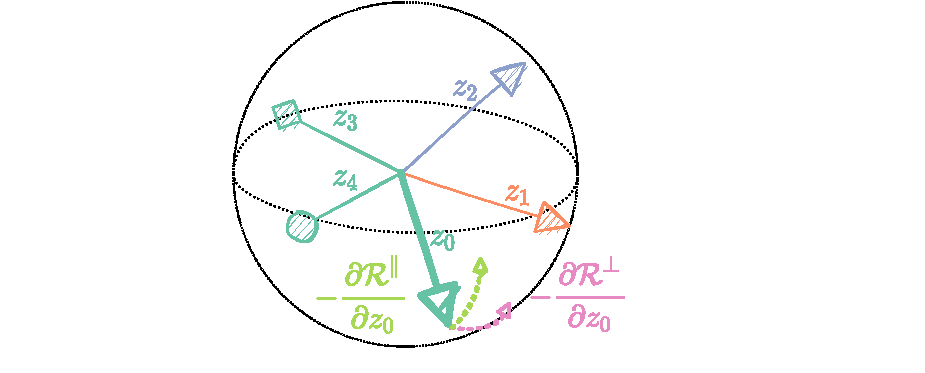
\includegraphics[width=0.6\columnwidth,trim={110 10 140 0},clip]{img/notation.pdf}
    \caption{Effect of the regularization term \eqref{eq:end-full-new} with respect to $z_0$. The features extracted from samples belonging to the same target class (same arrow's vertex) are entangled through the $R^\parallel$ term (in light green) while features for the same bias class (same color-in this case, with respect to $z_0$, dark green) are disentangled through the $R^\perp$ term (in pink).}
    \label{fig:notation}
\end{figure}
To visualize the effect of $\mathcal{R}$ as expressed in Eq.~\ref{eq:end-full-new}, consider a simple classification problem with three target classes and three different bias as illustrated in Fig.~\ref{fig:notation}. %
Training a model without explicitly addressing the presence of biases in the data, will most likely results in representations aligned by the bias attributes rather then the actual target class (Fig.~\ref{fig:notation}). 
The goal of $\mathcal{R}$ is to encourage the alignment of representations based on the correct features by \emph{i.)} disentangling representations of the same bias ($\mathcal{R}^\perp$) and \emph{ii.)} entangling representations of the same target in order to introduce invariance to the bias features ($\mathcal{R}^\parallel$).

